\documentclass[ignorenonframetext]{beamer}
\usepackage{beamerthemesplit}
\usepackage{amssymb}

%\documentclass[a4paper]{article}
\usepackage{beamerarticle}
\usepackage{verbatim}

\usepackage{../fhnw-beamer}

%\mode<article>{\usepackage{fullpage}}
%\mode<presentation>{\usetheme{Berlin}}

\date{\today}
\author{rolf.schmutz@fhnw.ch}
\institute{FHNW}
\title {Netzwerke und Datenkommunikation\\B-LS-MI 004\\Physical Layer}


\begin{document} % ===============================================================

\section{NDK B-LS-MI 004: L1}



\begin{frame}
\titlepage
\end{frame}

\begin{frame}
\frametitle{Ziele}
\begin{itemize}
	\item{Repr\"asentation des Quellsignals auf elektromagnetischer Ebene}
	\item{Codierung des Quellsignals (Abgek\"urzt)}
	\item{Verfahren zur Leitungscodierung der Daten aus einem Quellenstrom}
	\item{Techniken in Bezug auf Basisband- und Breitband-Kommunikation (Modulation)}
	\item{Fehlererkennung und -Korrektur}
\end{itemize}
\end{frame}


\frame { %------------------------------------------
\frametitle{Layer 1: Physical Layer}
\begin{itemize}
\item Der \emph{Physical Layer} ist f\"ur die bitweise \"Ubertragung der
	Daten verantwortlich.
\item Es werden Eigenschaften in den folgenden Gebieten definiert:
\begin{itemize}
\item Mechanische (Pinbelegungen, Stecker)
\item \"Ubertragungsart  (Elektrisch, Optisch, RF, Modulation oder Basisband, Seriell oder Parallel)
\item Prozedurale und Funktionale Abl\"aufe
\end{itemize}
\end{itemize}
}





\begin{frame}
\frametitle{Einfachste Bit-Serielle Daten\"ubertragung}
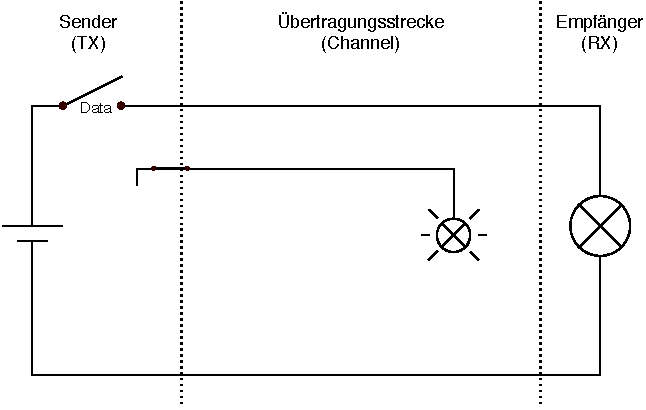
\includegraphics{simplest-serial}

\begin{itemize}
  \item ``Hello World!'' soll \"ubertragen werden
\end{itemize}
\end{frame}
%% Linu/URL/referenz: \myurl{http://www.rfc-editor.org/rfc/pdfrfc/rfc1918.txt.pdf}


\begin{frame}
\frametitle{Probleme}
\begin{itemize}
  \item wie wird ``Hello World!'' als Abfolge von Licht/kein-Licht (0, 1) dargestellt? (Quellcodierung)
  \item wann beginnt die Nachricht, einzelne Buchstaben, einzelne Bits, wann enden sie?
  \item wie k\"onnen einzelne gleiche ``bits'' getrennt werden? z.B. ``o''=01101111
\end{itemize}
\end{frame}


\begin{frame}
\frametitle{Quellencodierung (source-coding) 1/2}
\begin{block}{}
  Das ist die Repr\"asentierung von Informationen in bin\"arer (numerischer) Form, 
  also nicht Programm-Quellcode/sourcecode
\end{block}

\begin{itemize}
  \item es wird eine \"Ubereinkunft/Tabelle ben\"otigt, die die Information in numerischer Form (Bitmuster) festlegt (code-point)
  \item es gibt eine Vielzahl von Codierungen f\"ur verschiedene Datenformate
\end{itemize}
  \begin{block}{}{Die Codierung muss auf beiden Seiten bekannt sein und ist nicht gleich ``Verschl\"usselung''}\end{block}
\end{frame}

\begin{frame}
\frametitle{Quellencodierung (source-coding) 2/2}

F\"ur unsere Zwecke benutzen wir die alterw\"urdige ASCII-Codierungstabelle (ohne Kontrollzeichen):

\begin{center}
\begin{tabular}{l|l}
\begin{minipage}{5cm}
   \begin{tiny}\verbatiminput{asciitable.txt}\end{tiny}
\end{minipage} & z.B. ``H'': 48_{16} = 0100'1000_{2} \\
\end{tabular}
\end{center}

\end{frame}


\begin{frame}
\frametitle{Bit-Synchronisation: Strobe/Clock/Sampling (1/2)}
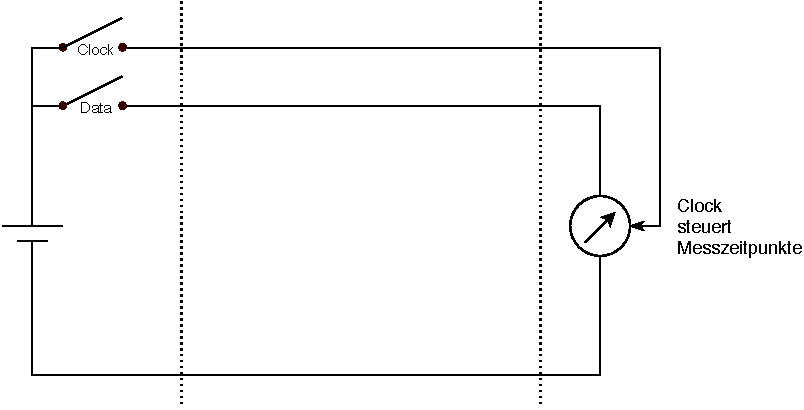
\includegraphics{simplest-serial-clock}
\end{frame}


\begin{frame}
\frametitle{Bit-Synchronisation: Strobe/Clock/Sampling (2/2)}
\begin{itemize}
  \item mit der ``Clock'' Leitung wird dem Empf\"anger der korrekte Messzeitpunkt signalisiert
  \item Folgen von ``gleichen'' Bits (alles 0 oder alles 1) k\"onnen problemlos getrennt werden
\end{itemize}
\begin{block}{Synchrone Bitserielle \"Ubertragung}
Es werden mindestens drei Leitungen ben\"otigt, daf\"ur sind keine weiteren Massnahmen n\"otig.

Synchrone Daten\"ubertragung wird vorallem im Nahbereich (im Computer, Embedded Systems I^{2}C/SPI, HDMI, etc) eingesetzt
\end{block}
\begin{itemize}
  \item es kann auch zwischen ``keine Daten'' (Clock=0) und ``0'' Bits unterschieden werden
\end{itemize}
\end{frame}


\begin{frame}
\frametitle{Asynchrone Serielle \"Ubertragung (1/3)}
Eine weitere M\"oglichkeit eine Synchronisierung\footnote{wenn auch im Titel ``Asynchron''} ist das ``Framing'' der \"Ubertragung

\begin{itemize}
\item eine Startsequenz (Startbit oder Preamble) und eine optionale Endsequenz werden in den Datenstrom eingef\"ugt\footnote{dies sind bereits keine ``Nutzdaten'' mehr sondern Teil des Protokolls}
\item der Empf\"anger hat damit die M\"oglichkeit, sich \emph{f\"ur die Dauer der Nachricht/Zeichens} mit dem Sender zu synchronisieren
\item mit dem Framing kann beim Empf\"anger auch zwischen Daten/keine-Daten unterschieden werden (ausserhalb des Frames werden Daten ignoriert)
\end{itemize}
\begin{block}{Asynchrone Bitserielle \"Ubertragung}
Es werden nur zwei Leitungen/ein Kanal ben\"otigt. Daf\"ur ist die Methode ein wenig aufwendiger zu implementieren.
\end{block}
\end{frame}



\begin{frame}
\frametitle{Asynchrone Serielle \"Ubertragung (2/3)}
Bei einfachen seriellen Schnittstellen\footnote{RS232 und \"aquivalent} wird ein Startbit (optional Stopbit) eingef\"ugt, {\bfseries jedes Byte/Zeichen wird einzeln synchronisiert}

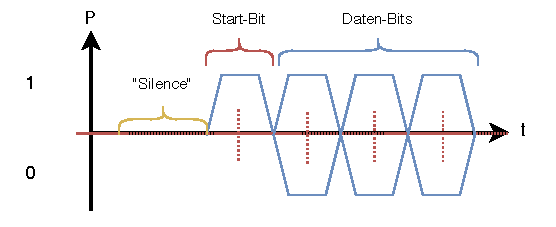
\includegraphics[height=3cm]{asynchron-startbit}
\begin{itemize}
\item der Empf\"nger muss ungef\"ahr die Transferrate/Bitzeit schon kennen und kann das Sampling nach dem Startbit einstellen
\item die M\"oglichkeit einer Startsequenz ``10'' vereinfacht dies weiter
\item moderne Implementationen buffern die \"Ubertragung ein paar bits und k\"onnen damit ``autobaud'' -- selbst\"andige Adaption an die Datenrate implementieren
\end{itemize}
\end{frame}


\begin{frame}
\frametitle{Asynchrone Serielle \"Ubertragung (3/3)}
Bei ``Ethernet'' (der Quasi-Standard im Internet/IP-Netzwerken) wird mit einer Pr\"aambel gearbeitet
\begin{itemize}
\item 7 Bytes $AA_{16}$ + 1 Byte $AB_{16}$ {} (d.h. insgesamt 64 Bit)
\item der Empf\"anger hat eine eigene Clock-Source mit der ungef\"ahren Frequenz aber unbekannter Phase. \"Uber eine PLL wird die korrekte Phase ermittelt:
\end{itemize}
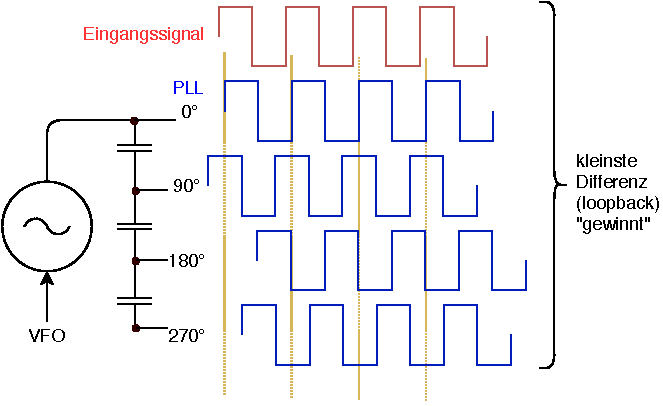
\includegraphics[height=5cm]{asynchron-ethernet}
\end{frame}


\begin{frame}
\frametitle{Interlude}
Damit w\"are das Problem ``Clock'' gel\"ost.

Wenn anstelle einer einfachen Lampe aber ein datenverarbeitendes System der
Empf\"anger ist, stellt sich eine weitere Frage:

\begin{block}{}
Wann ist ein Bit als ``1'' und wann als ``0'' zu interpretieren?
\end{block}
\end{frame}







\begin{frame}
\frametitle{Interpretation von Pegelbasierten Signalen (1/3)}
Eine \"Ubereinkunft kann mithilfe eines Schwellwerts (threshold) erreicht werden:

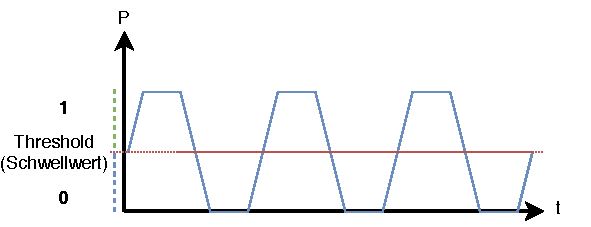
\includegraphics{threshold}

Dies geh\"ort nat\"urlich auch zur Protokolldefinition auf Schicht 1
\end{frame}





\begin{frame}
\frametitle{Interpretation von Pegelbasierten Signalen (2/3)}
Das Problem dabei ist eine abschw\"achung des Signals auf der Leitung (D\"ampfung), damit kann ein knappes Signal ``flackern'' und nicht eindeutig einem Wert zugewiesen werden:

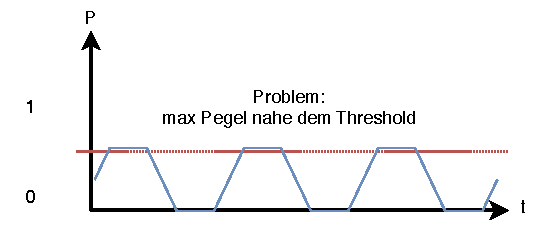
\includegraphics{threshold-soso}
\end{frame}


\begin{frame}
\frametitle{Interpretation von Pegelbasierten Signalen (3/3)}
Abhilfe schafft ein sogenannter Schmitt-Trigger\footnote{in fast allen Pegelbasierten Systemen so implementiert}

\vspace{0.5cm}

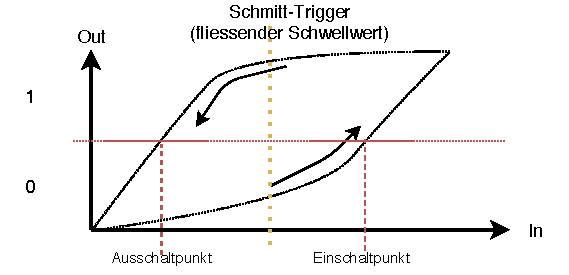
\includegraphics{schmitt-trigger}
\end{frame}


\begin{frame}
\frametitle{Nicht-Pegelbasierten Signale}
\begin{itemize}
  \item Phasenlage\footnote{relative...}: wird durch D\"ampfung nicht beeinflusst
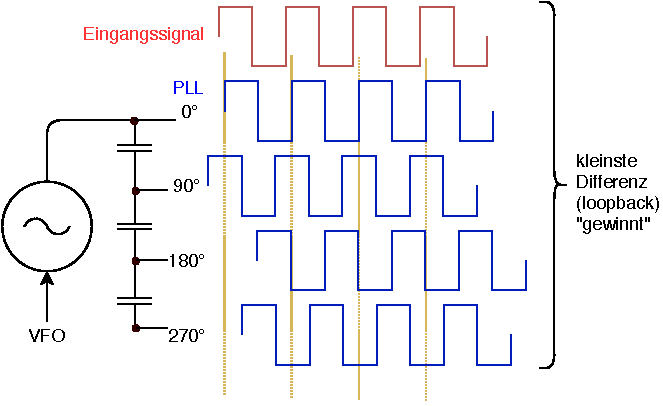
\includegraphics[height=1.5cm]{asynchron-ethernet}

  \item Nulldurchg\"ange/Flanken: Richtung der Flanke (up/down) wird ebenfalls nicht durch D\"ampfung beeinflusst und ist sehr robust zu detektieren\footnote{``Manchester''-Code}

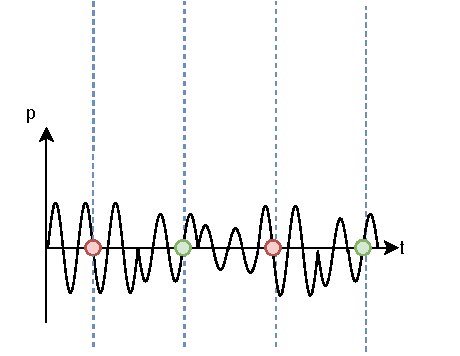
\includegraphics[height=3cm]{zero-crossing}
\end{itemize}
Diese Techniken werden unter ``Multiplexing'' vertieft.
\end{frame}




\begin{frame}
\frametitle{Interlude}
Damit sind nun die Fragen:

\begin{itemize}
  \item wann soll gemessen werden?
  \item wie soll die Messung interpretiert werden?
\end{itemize}
gekl\"art.

\begin{block}{Diskriminator}
Solche Schaltungen, die ein Signal quantisieren (in zwei oder mehr Werte) werden auch {\bfseries Diskriminatoren} genannt
\end{block}
\end{frame}



\begin{frame}
\frametitle{Line-Coding Basisband/Baseband: Blockschaltbild}
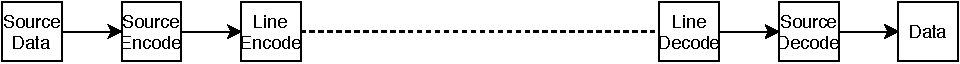
\includegraphics[width=12cm]{baseband-circuit}
\begin{itemize}
  \item Source-Data sind die zu \"ubertragenden Daten. Dies kann auch eine ``analoge'' Quelle sein.
  \item Source-Encode/Decode: wie wird die Information r\"apresentiert/interpretiert. z.B. ASCII-Table
  \item Line-Code/Decode: wie wird die numerische/bin\"are Information als elektromagnetisches Signal r\"apresentiert/interpretiert
\end{itemize}
\begin{block}{}
Es muss eine \"Ubereinkunft \"uber die verwendeten Codierungen\footnote{deshalb ``nicht-geheim''} stattfinden. Line-Code geh\"ort zur Schicht 1.
\end{block}
\end{frame}


\begin{frame}
\frametitle{Baseband: Codierungen}
\begin{small}
\begin{itemize}
  \item NRZ: Basis-Schema: Gleichstromfalle
  \item NRZI: \"Anderungen nur bei einem ``1'' Bit: Transition und nicht Pegel
  \item Bipolar: kann auch ``keine Daten'' signalisieren
  \item Manchester: Flanken/Nulldurchgang codiert: Taktfrequenz ableitbar, kein Gleichstrom
\end{itemize}
\end{small}
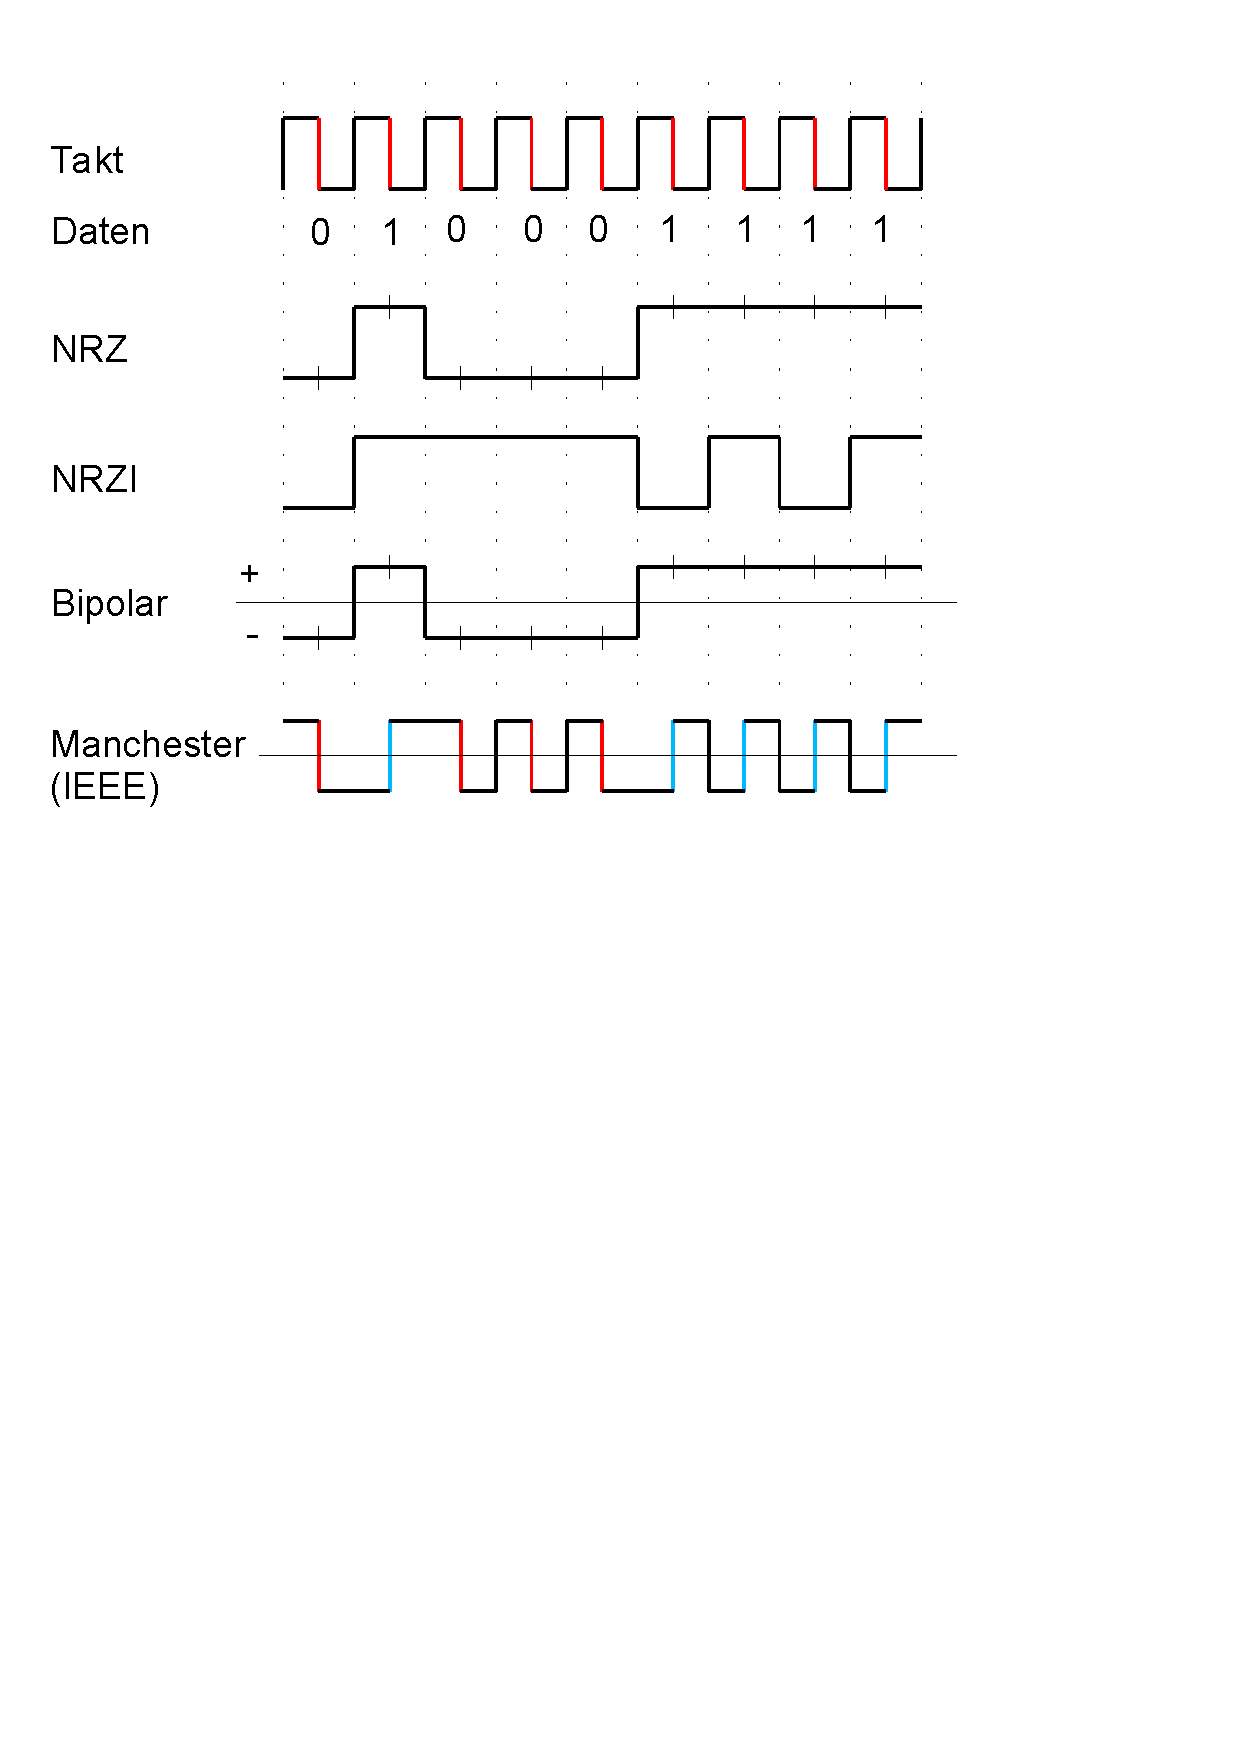
\includegraphics[height=10.5cm]{bitcodes}

\end{frame}



\begin{frame}
\frametitle{Multiplexing/``Broadband'' (1/7)}
Bisher wurde angenommen, dass die \"Ubertragung \"uber Leitungen (galvanisch, optisch) ``exklusiv'' erfolgt.
\begin{block}{Duplex/Multiplex}
Was nun, wenn \"uber zwei Dr\"ahte mehr als ein ``Kanal'' implementiert werden soll?\footnote{z.B. Radio-/Fernsehkan\"ale Broadcast oder eine Modem-Strecke Duplex senden/empfangen auf der selben Leitung} Oder gar keine gleichstrom-f\"ahige Leitung zur Verf\"ugung steht (Radioband, Modemleitungen)
\end{block}

Dazu muss ein {\emph Multiplexing}-Verfahren eingerichtet werden. Eine solche \"Ubertragung (FDM) wird als ``Broadband'' bezeichnet.
\end{frame}




\begin{frame}
\frametitle{Multiplexing (2/7)}
\begin{columns}
\begin{column}{3cm}
\begin{center}
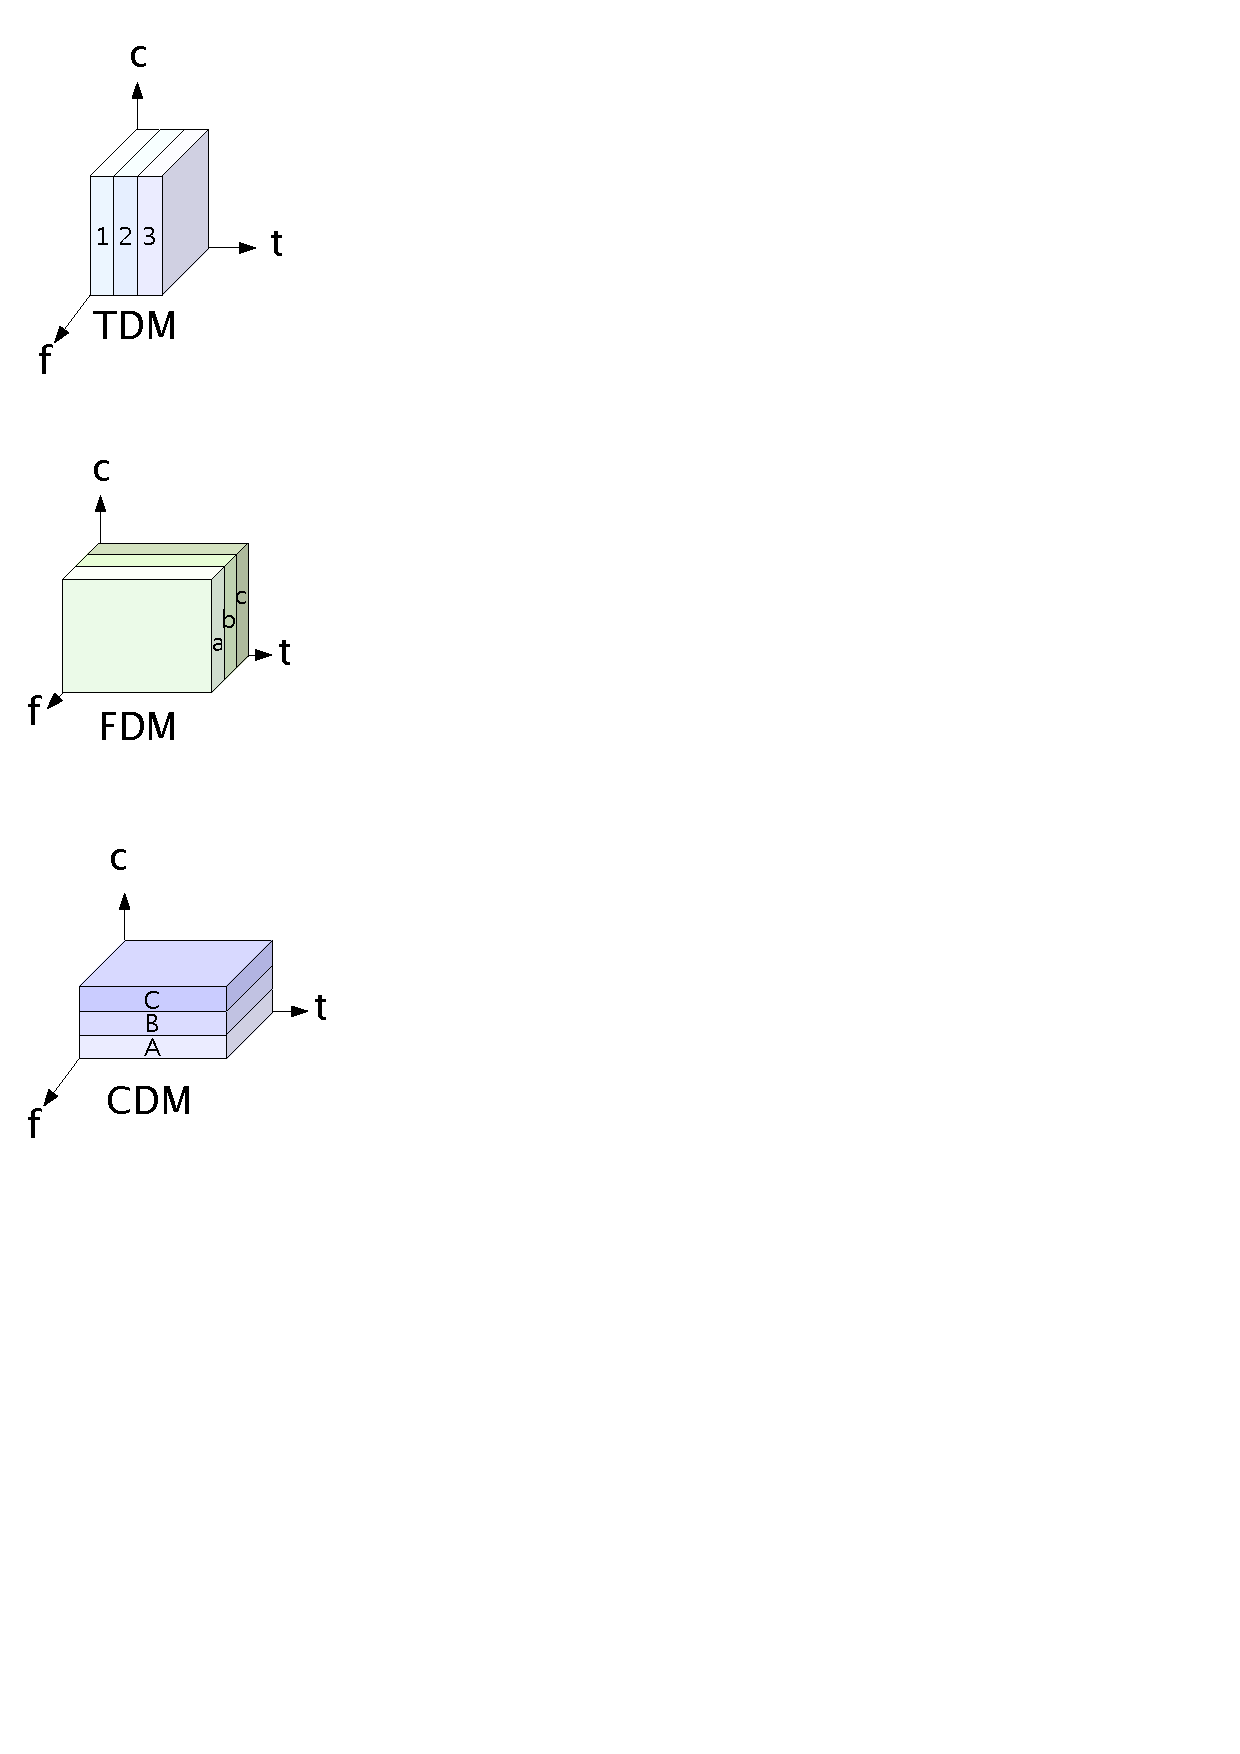
\includegraphics[width=0.7\textwidth]{multiplex}
\end{center}
\end{column}
\begin{column}{8cm}
\begin{itemize}
\item[TDM:] Time Division Multiplex: Die Kan\"ale werden zeitlich abwechselnd auf
	der selben Leitung \"ubertragen
\item[FDM:] Frequency Division Multiplex: Die Kan\"ale werden auf verschiedenen Frequenzen
	auf der selben Leitung \"ubertragen
\item[CDM:] Code Division Multiplex: Die Kan\"ale werden gleichzeitig mit verschiedenen
	Codes \"ubertragen
\end{itemize}
\end{column}
\end{columns}
\end{frame}







\begin{frame}
\frametitle{Multiplexing: TDM (3/7)}
Time-Division\footnote{oder ``Domain''} Multiplexing weist zeitlich getrennt (``Zeitschlitze'') einen \"Ubertragungskanal\footnote{normalerweise im Basisband, aber auch \"uber FDM-Kan\a"le \"ublich: WLAN, Funkamateure, etc} verschiedenen Quellen zu. 

Dabei kommen verschiedene Techniken zum Einsatz:
\begin{itemize}
  \item statisches Multiplexing: eine gewisse Anzahl Sender/Empf\"anger ist fest eingestellt und es wird ein ``Schalter'' f\"ur die jeweilige Paarung synchron auf Mux/Demux rotiert
  \item dynamisches Multiplexing: gleiche Voraussetzungen aber mit adaptivem Verhalten -- nicht genutzte Kan\"ale werden \"ubersprungen
  \item kooperatives Multiplexing: z.B. CSMA/CD von Ethernet: ein Sender darf nur nach einer gewissen ``Ruhephase'' des Mediums zu senden beginnen. Das ausgesendete Signal wird dabei vom Sender auf St\"orungen (ein anderer Sender) \"uberwacht und bei St\"orung abgebrochen\footnote{das f\"uhrt zu keiner deterministischen Datenbandbreite funktioniert aber im Normalfall effizienter}
\end{itemize}
\end{frame}







\begin{frame}
\frametitle{Multiplexing: FDM (4/7)}
Es werden mehrere exklusive Kan\"ale auf dem geteilten Medium eingerichtet. Dazu wird das Nutzsignal zus\"atzlich auf eine Tr\"agerwelle \emph{aufmoduliert}\footnote{z.B. Radio-/Fernsehkan\"ale, WLAN}
\vspace{0.5cm}

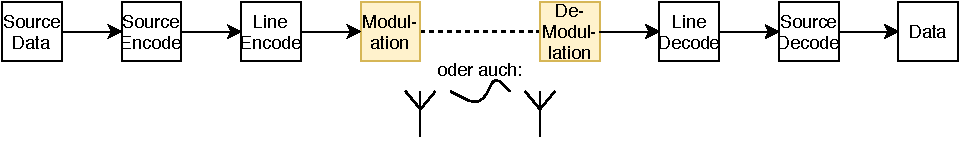
\includegraphics[width=12cm]{broadband-circuit}
\begin{block}{}
Die Modulation kann kontinuierlich (analog) oder in Schritten (quantisiert) erfolgen. Bei der digitalen Daten\"ubermittlung wird als ``\{Amplitude,Frequency,Phase\}-Shift-Keying'' bezeichnet.
\end{block}
\end{frame}





\begin{frame}
\frametitle{Multiplexing: FDM (5/7)}
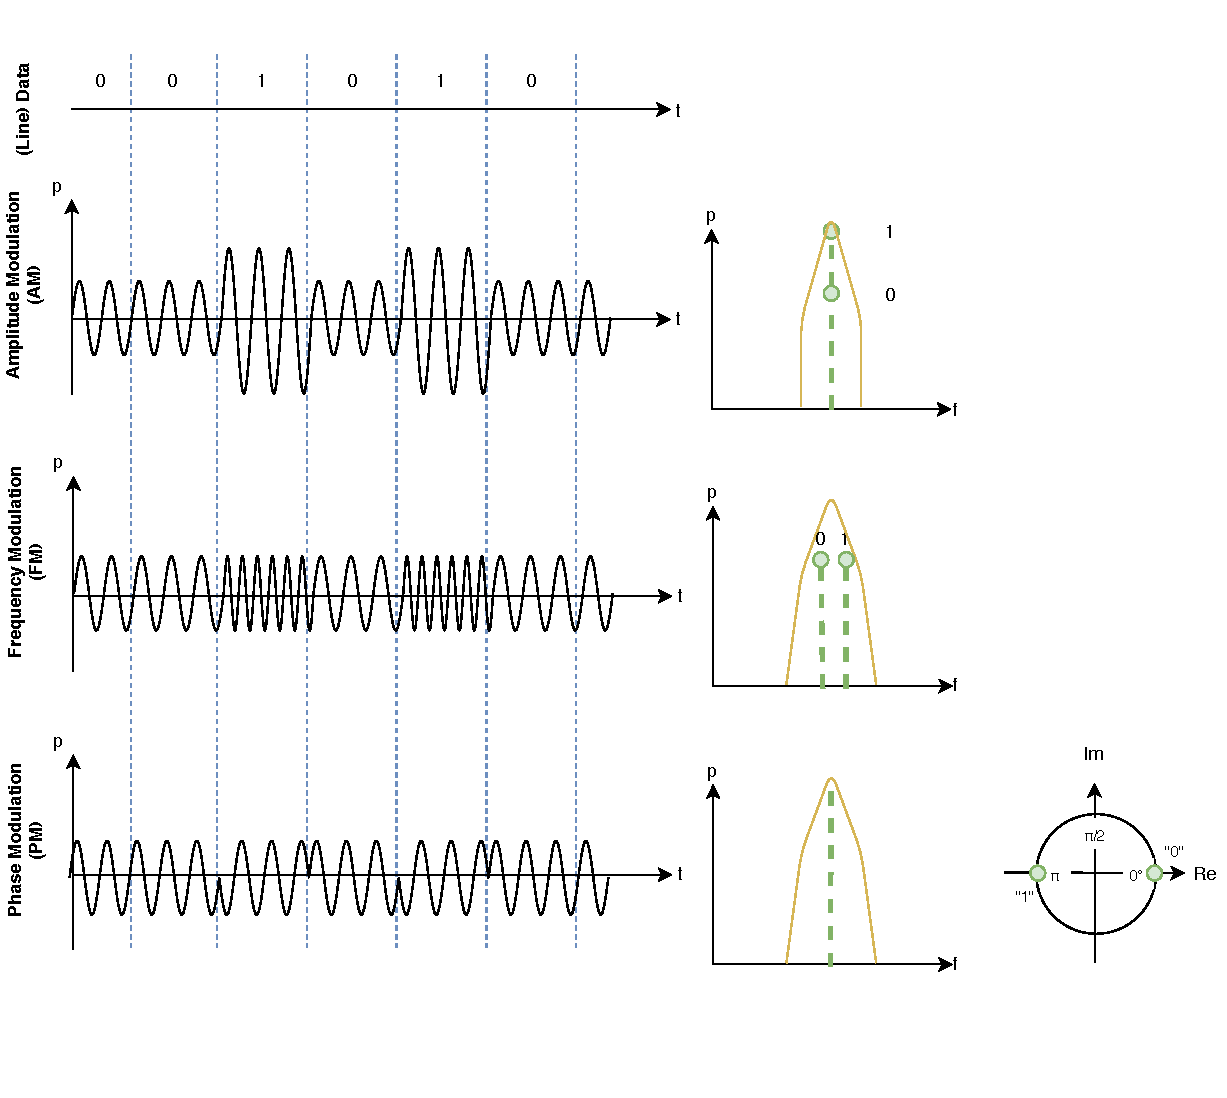
\includegraphics[height=9cm]{modulation-schemes}
\end{frame}





\begin{frame}
\frametitle{Multiplexing: FDM (5/7)}
Bei allen \"Ubertragungsarten sind auch ``Multi-Level''-Codierungen m\"oglich:


\begin{itemize}
  \item es kann mehr als ein Bit pro Sampling-Point \"ubertragen werden
  \item durch die vielen \"Uberg\"ange beim Signalverlauf entsteht ein ``breiteres'' Spektrum
  \item \{\_,A,Q\}-PSK und FSK sind aber ``robust''\footnote{Phasenlage und Frequenz wird nicht beeinflusst} gegen\"uber Verzerrungen durch Bandbreitenbeschr/"ankung
\end{itemize}

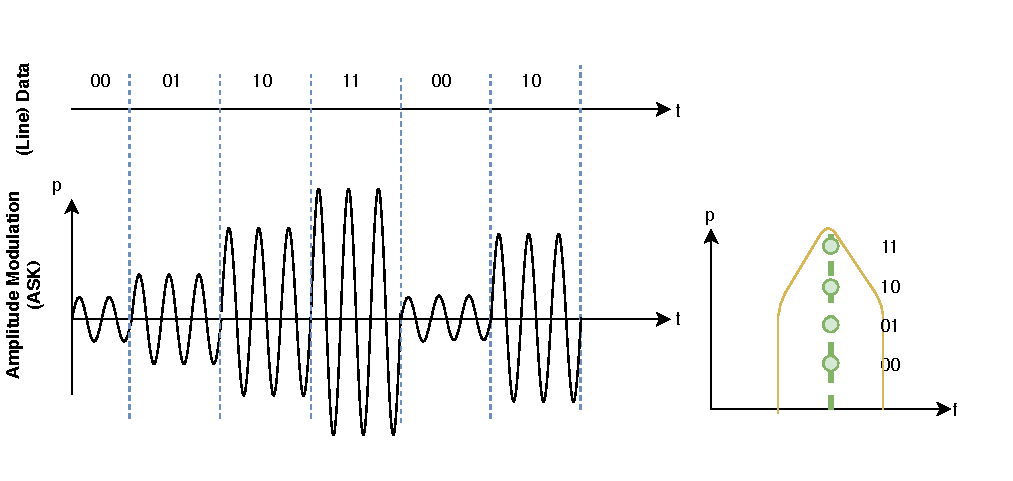
\includegraphics[width=10cm]{multilevel}
\end{frame}







\begin{frame}
\frametitle{Multiplexing: FDM (6/7)}
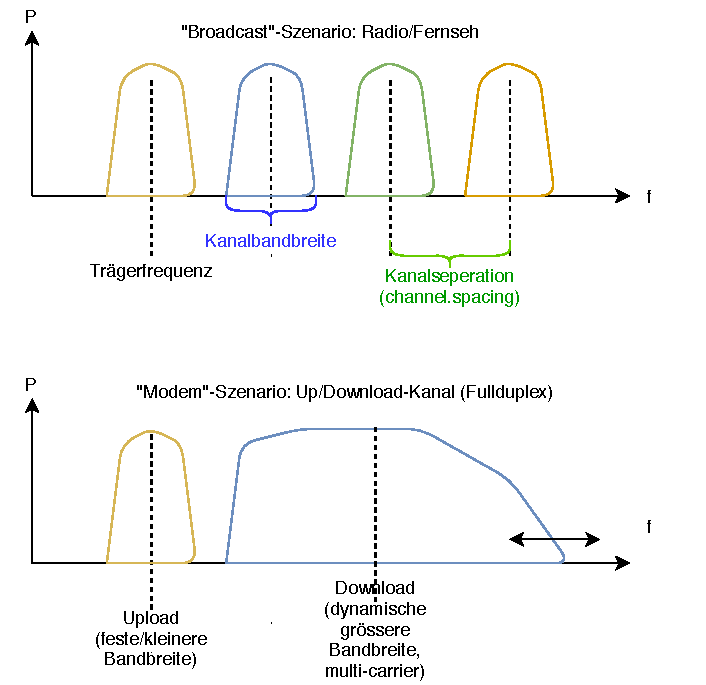
\includegraphics[height=8cm]{fm-spectra}
\end{frame}








\begin{frame}
\frametitle{Interlude}

\myurl{http://websdr.ewi.utwente.nl:8901}

Mit einem Multiplex-Verfahren kann ein Physikalischer Kanal\footnote{galvanisch, galvanisch-entkoppelt, Radiofrequenzen, optischer Link} in virtuelle ``Sub-Kan\"ale'' unterteilt werden. 

\begin{tiny}silly analogy ahead...\end{tiny}
\begin{itemize}
  \item TDM: Fernseh-/Radioprogramm: jede Sendung hat den Kanal exklusiv w\"ahrend einer bestimmten Zeitdauer
  \item FDM: Fernseh-/Radioprogramm: alle Sender k\"onnen gleichzeitig auf ``ihrem'' Kanal\footnote{``virtuell'' aufmoduliert auf eine bestimmten Tr\"agerfrequenz, mit bestimmter Bandbreite} senden 
\end{itemize}
\end{frame}









\begin{frame}
\frametitle{Limitation Elektromagnetischer \"Ubertragung (1/2)}
{\bfseries Jede} physikalische \"Ubertragungsstrecke unterliegt folgenden Limitationen:

\begin{itemize}
  \item verf\"ugbare physikalische Bandbreite\footnote{eigentlich aus dem Ersatzschaltbild ersichtlich} 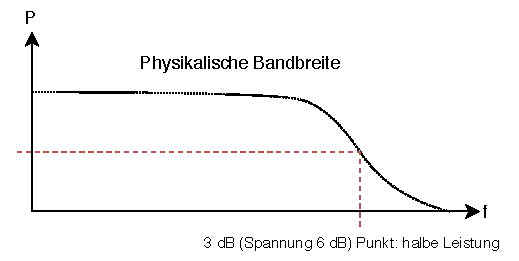
\includegraphics[height=3cm]{bandwidth}
  \item D\"ampfung des Signals (auch Frequenzabh\"angig) 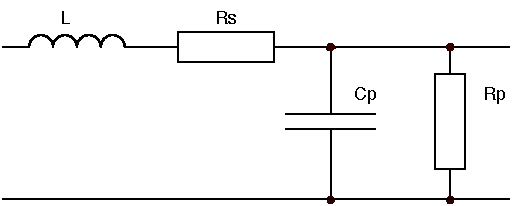
\includegraphics[height=3cm]{line-circuit}
\end{itemize}
\end{frame}



\begin{frame}
\frametitle{``Twisted-Pair'': Telegraphenleitung}
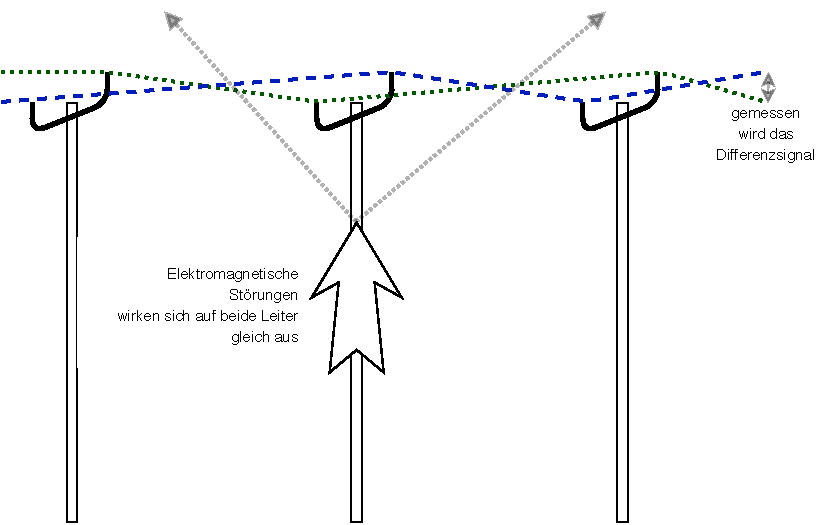
\includegraphics[width=11cm]{telegraph-line}
\end{frame}



\begin{frame}
\frametitle{Twisted-Pair: TP-Leitungen}
\framesubtitle{Kabel / RJ-45 Stecker}


\begin{itemize}
\item [UTP] Unshielded Twisted Pair: g\"unstig, physikalisch stabil, bis ca. 50m
Die meisten Netzwerkkabel mit RJ-45 Stecker f\"ur Ethernet
	enthalten 8 isolierte Leiter in vier Paaren verdrillt. Bis 
	100MBit/s werden nur zwei Paare ben\"otigt.
	Bei Patchkabeln sind alle Adern der Stecker 1:1 verbunden,
	bei Crossover-Kabeln sind sie ausgekreuzt.
\item [STP] Shielded Twisted Pair: Die einzelnen Aderpaare (FTP:
 Folied Twisted Pair)  sind bzw. auch noch 
	das ganze Kabel (S/FTP: Screened Foiled Twisted Pair) sind
	 zus\"atzlich zur Verdrillung abgeschirmt), teuerer als UTP, 
	 l\"angere Leitungsl\"angen m\"oglich (bis ca. 100m), bessere EMV.

\item [CAT5] Kabelklasse, welche bis 100 MBit/s verwendet wird.
\end{itemize}
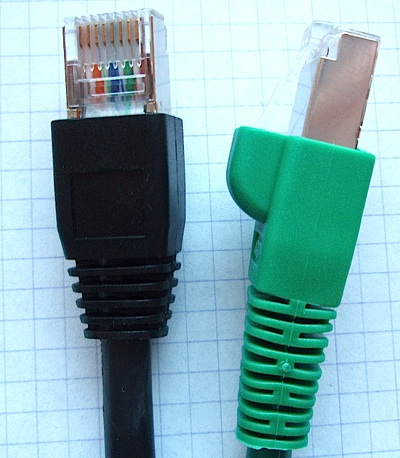
\includegraphics[width=2.5cm\textwidth]{rj45Stecker.jpg}
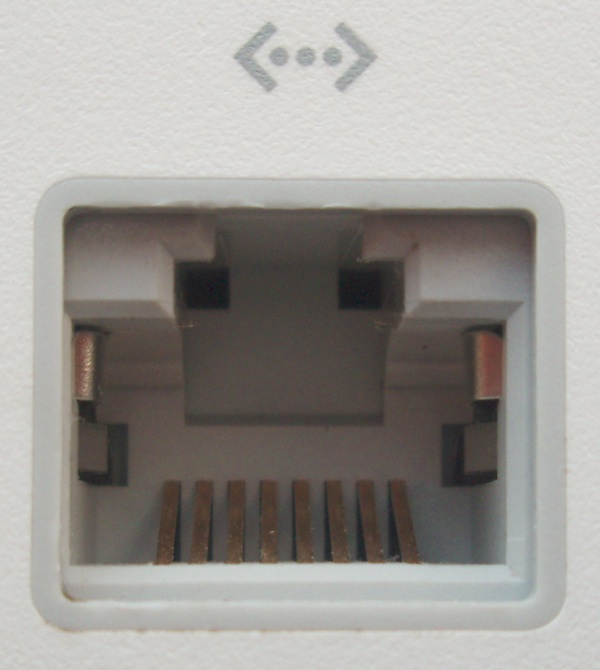
\includegraphics[width=2.5cm\textwidth]{rj45Buchse.jpg}

\end{frame}




\frame { %------------------------------------------
\footnotetext[1]{\tiny{A. Tanenbaum, ''Computer Networks'', http://authors.phptr.com/tanenbaumcn4/}}
\frametitle{Weitere \"Ubertragungsmedien}
\begin{columns}
\begin{column}{5.5cm}
\begin{figure}
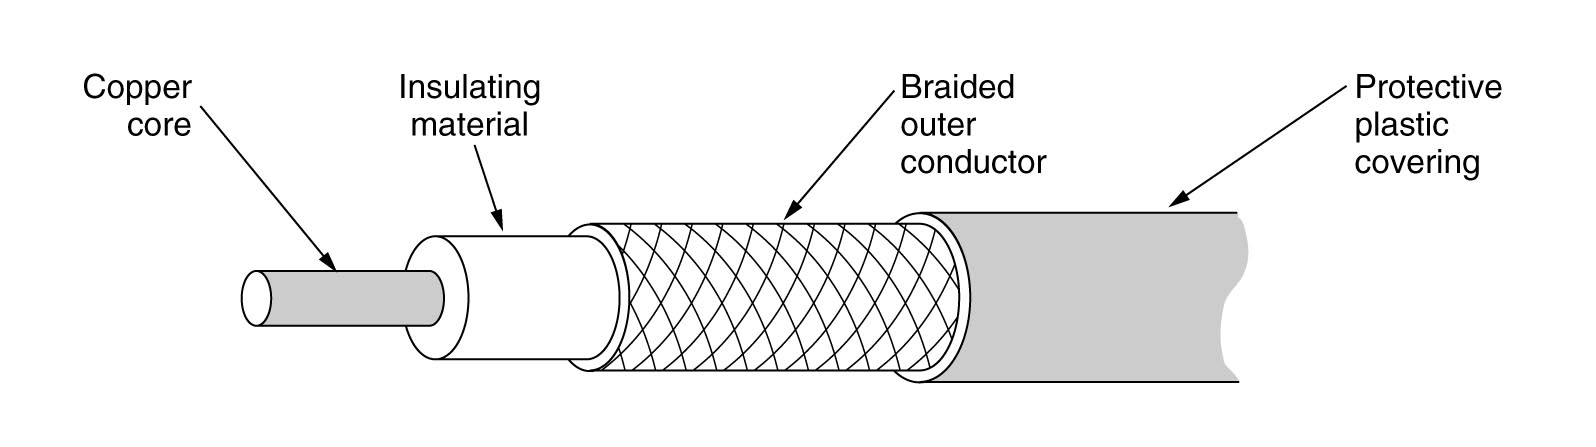
\includegraphics[width=0.9\textwidth]{2-04.jpg}
\caption{ \tiny{2-04\footnotemark[1], Koaxial-Kabel}}
\end{figure}
\begin{figure}
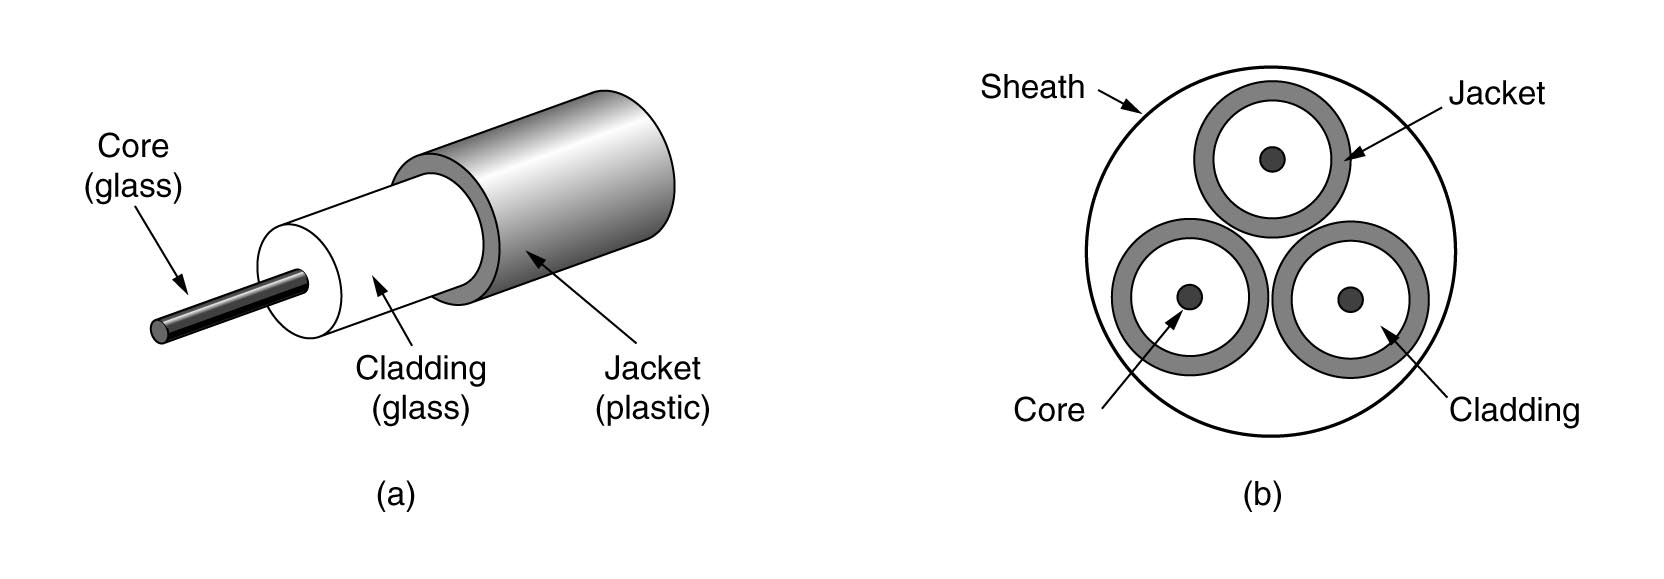
\includegraphics[width=0.9\textwidth]{2-07.jpg}
\caption{ \tiny{2-07\footnotemark[1], LWL}}
\end{figure}
\end{column}
\begin{column}{5.5cm}
\begin{figure}
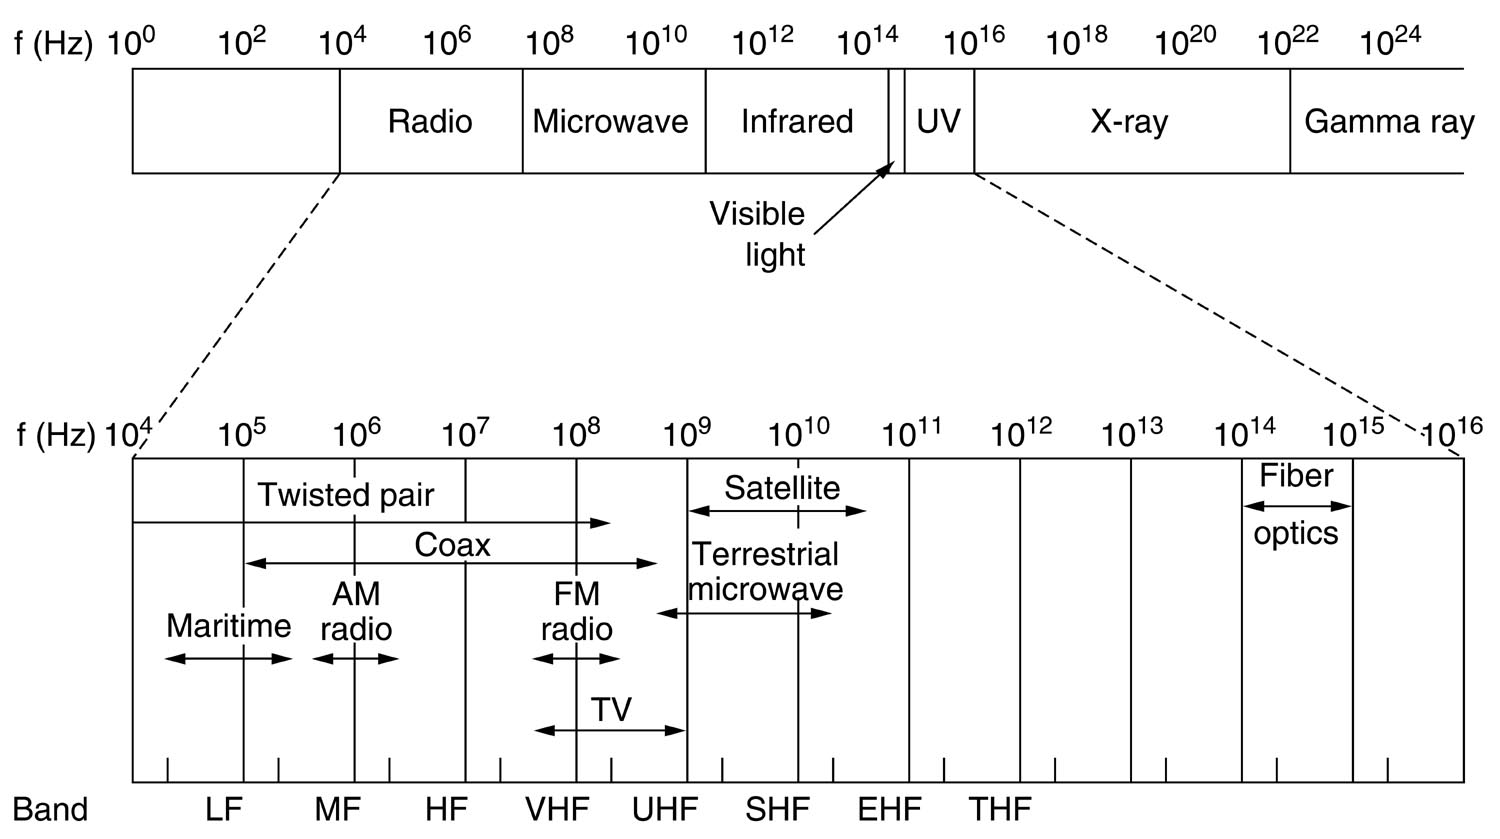
\includegraphics[width=0.7\textwidth]{2-11.jpg}
\caption{ \tiny{2-11\footnotemark[1], Frequenzspektrum}}
\end{figure}
\begin{figure}
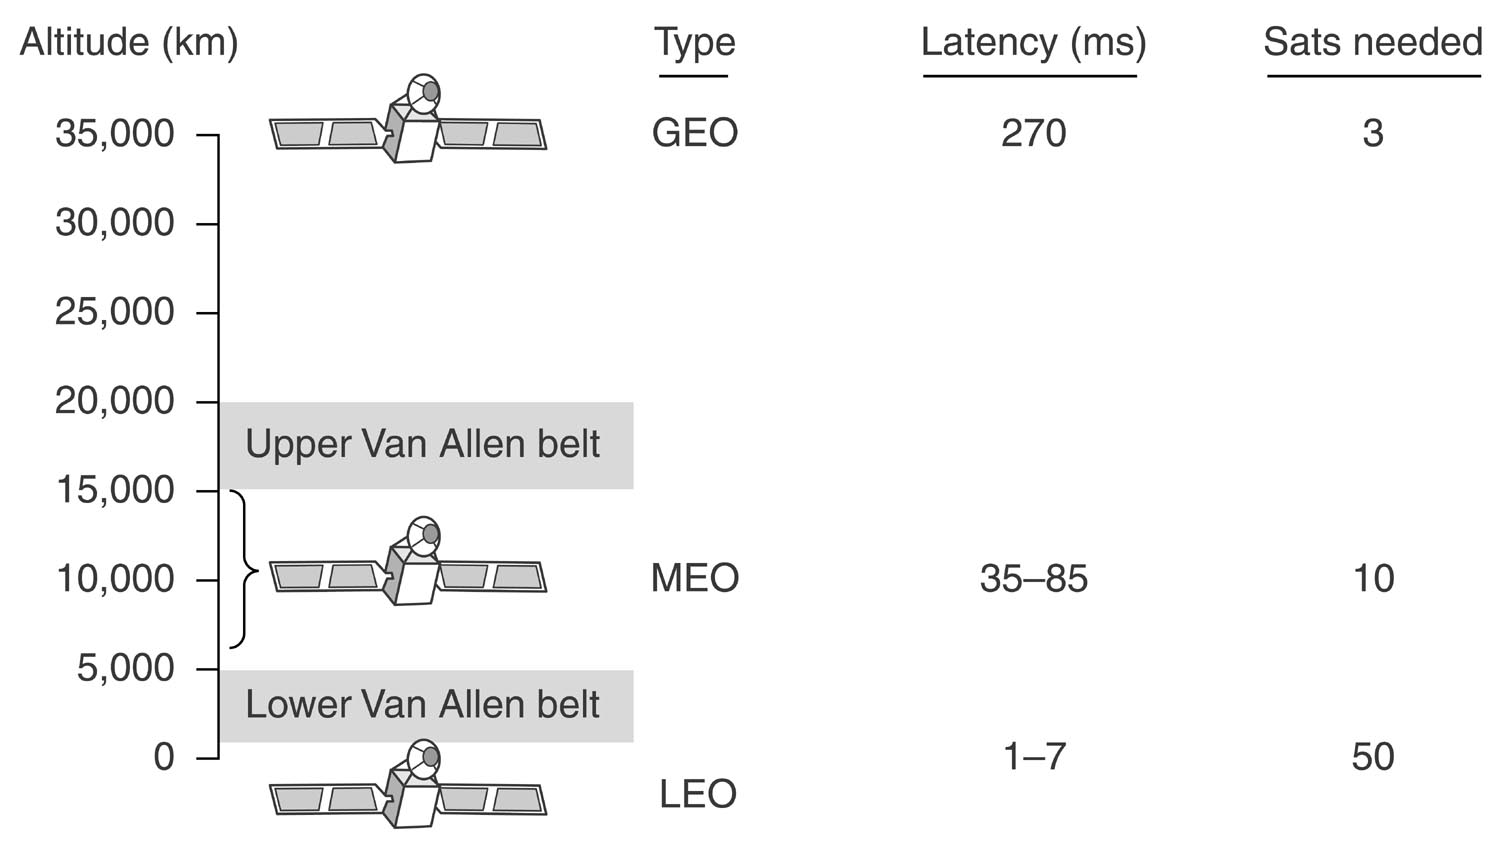
\includegraphics[width=0.6\textwidth]{2-15.jpg}
\caption{ \tiny{2-15
\footnotemark[1], Satelliten}}
\end{figure}
\end{column}
\end{columns}
}


\frame { %------------------------------------------
\frametitle{L1:  \"Ubertragungsmedien 3/4}
\framesubtitle{Verluste/D\"ampfung}
Beim Einsatz von Kupferkabeln muss bei der \"Ubertragung immer
mit Verlusten gerechnet werden. Verluste entsprechen einer
\alert{D\"ampfung} und werden in \alert{dB} angegeben.
Dabei gilt f\"ur das Verh\"altnis zwischen Eingangs- und Ausgangs\alert{spannung}:
  \begin{displaymath}
  a = 20\log \left(\frac{V2}{V1}\right)
  \end{displaymath}
{\tiny \textit{a: D\"ampfung in dB, V2: Ausgangsspannung, V1 Eingangsspannung}}\\
Zus\"atzlich ist es bei Kabeln interessant, wie stark die einzelnen
Leitungspaare einander beeinflussen, dies wird z.B. mit dem \alert{NEXT}
(Near End Crosstalk) Wert angegeben (+Weitere Parameter).
\begin{center}
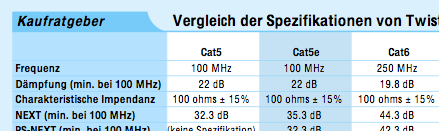
\includegraphics[width=0.4\textwidth]{next.png}  
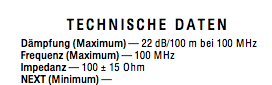
\includegraphics[width=0.4\textwidth]{daempfung.png} 
\end{center}
\small Siehe auch: \myurl{http://www.netzmafia.de/skripten/netze/netz6.html\#6.1}
}


\frame { %------------------------------------------
\frametitle{L1:  \"Ubertragungsmedien 4/4}
\framesubtitle{Lichtwellenleiter / Glasfaser}
\small
%Die heute immer vermehrt eingesetzten Lichtwellenleiter in der
%Vernetzungstechnik sind noch immer einiges teuerer als die 
%herk\"ommlichen Kupferkabel, bieten aber auch einige Vorteile:
\begin{itemize}
\footnotesize
\item LWL's sind viel st\"orungsunempfindlicher als Cu-Kabel, 
	es kann praktisch keine Fremdeinkopplung von St\"orsignalen 
	stattfinden.
\item Die Leitungsd\"ampfung ist praktisch frequenzunabh\"angig und 
	wesentlich tiefer als bei Cu-Kabeln.
\item Die \"Ubertragungskapazit\"at in LWL's ist ist gr\"osser als die von
	Cu-Kabeln (bis in den GBit/s Bereich). Es k\"onnen	unterschiedliche Wellenl\"angen parallel verwendet werden.
\end{itemize}
Bei LWL's werden verschiedene Typen unterschieden:
\begin{description}
\footnotesize
\item[Monomode] Sehr d\"unne Faser, welche das Licht nur bei 
	einer bestimmten Wellenl\"ange gut leiten, es findet praktisch
	keine Reflexion am Cladding statt, es sind grosse Geschwindigkeiten
	und lange Leitungsl\"angen m\"oglich.
\item[Multimode] Leiten das Licht auf verschiedenen Wellenl\"angen,
	die Ausbreitung findet durch Reflexion am Cladding statt, daher
	ist die D\"ampfung etwas gr\"osser als bei Monomode-Fasern.
\end{description}

Siehe auch: \myurl{http://www.netzmafia.de/skripten/netze/netz5.html\#5.6}
}




\end{document}